\NeedsTeXFormat{LaTeX2e}
\documentclass[12pt,a4paper]{article}
\usepackage[includeheadfoot,margin=2.5cm]{geometry}
\usepackage{amssymb}
\usepackage{amsmath}
\usepackage{floatflt}
\usepackage{graphicx}
\usepackage{color}
\usepackage{subfig}
\usepackage[english,ngerman]{babel}
\usepackage{listings}
\usepackage{url}
\usepackage[T1]{fontenc}
\usepackage[utf8]{inputenc}
\usepackage{titlesec}
\usepackage{float}
\usepackage{enumitem}
\usepackage{subfig}
\usepackage[section]{placeins}
\usepackage[smaller]{acronym}
\usepackage[font=small,labelfont=bf]{caption}
\usepackage{tabularx}
\usepackage{multirow}
\usepackage{booktabs}
\usepackage{textcomp}

\usepackage{chngcntr}
\counterwithout{footnote}

\usepackage{tabu}
\usepackage{booktabs}% for better rules in the table

\usepackage{natbib}
\hyphenation{lastEventID}


\hyphenation{
    %add manual hyphenation rules in the format: Fach-hoch-schule
}

%Hyphenation Settings
%\clubpenalty=10000
%\widowpenalty=10000
%\displaywidowpenalty=10000
%\brokenpenalty10000\relax



\setlength{\parindent}{0pt}
\setlength{\parskip}{5pt plus 2pt minus 1pt}


\titleformat{\paragraph}{\normalfont\normalsize\bfseries}{\theparagraph}{1em}{}
\titlespacing*{\paragraph}{0pt}{3.25ex plus 1ex minus .2ex}{1.5ex plus .2ex}

\setcounter{secnumdepth}{3}
\setcounter{tocdepth}{3}


\lstset{
    language=C,
    basicstyle=\ttfamily,
    keywordstyle=\color{blue},
    tabsize=4,
    numbers=left,
    numberstyle=\footnotesize,
    breaklines=true,
%   morekeywords={*,auto}
}

\lstdefinelanguage{JavaScript}{
  keywords={typeof, new, true, false, catch, function, return, null, catch, switch, var, if, in, while, do, else, case, break},
  keywordstyle=\color{blue}\bfseries,
  ndkeywords={class, export, boolean, throw, implements, import, this},
  ndkeywordstyle=\color{darkgray}\bfseries,
  identifierstyle=\color{black},
  sensitive=false,
  comment=[l]{//},
  morecomment=[s]{/*}{*/},
  commentstyle=\color{purple}\ttfamily,
  stringstyle=\color{red}\ttfamily,
  morestring=[b]',
  morestring=[b]"
}

\selectlanguage{ngerman}



\begin{document}

\begin{titlepage}
\begin{center}


\includegraphics[width=5cm]{images/FHSLogo.jpg}

\vspace*{4cm}

\Large{
	\textit{
		\textbf{Asynchronous Programming in Ruby} 
		\linebreak 
		Is Ruby capable of doing asynchronous programming?
	}
}

\vspace*{4cm}

\large{
	\textbf{BACHELORARBEIT 2}
}

\end{center}

\vfill

\begin{tabbing}
StudentIn \= \ Thomas Mayrhofer, FHS34784 \\
BetreuerIn \> \ Mag. (FH) Hannes Moser
% uncomment the following line for an optional second supervisor:
%          \> \ Titel Vorname Familienname
\end{tabbing}

Puch Urstein, 9. April 2014
% uncomment the following 3 lines for an optional lock flag, max. 2 years!
%\hfill
%\color{red}
%\framebox{Sperrvermerk bis 20/01/2012}

\end{titlepage}

\pagestyle{headings}
\pagenumbering{roman}

\subsection*{Eidesstattliche Erklärung}

Hiermit versichere ich, Thomas Mayrhofer, geboren am {\bf 15.September 1992} in {\bf Linz}, dass ich die Grundsätze wissenschaftlichen Arbeitens nach bestem Wissen und Gewissen eingehalten habe und die vorliegende Bachelorarbeit von mir selbstständig verfasst wurde. Zur Erstellung wurden von mir keine anderen als die angegebenen Quellen und Hilfsmittel verwendet. 

Ich versichere, dass ich die Bachelorarbeit weder im In- noch Ausland bisher in irgendeiner Form als Prüfungsarbeit vorgelegt habe und dass diese Arbeit mit der den \mbox{BegutachterInnen} vorgelegten Arbeit übereinstimmt.


\vspace*{3cm}

{\bf Puch Urstein}, am {\bf 4. Mai 2015}


\hfill


Unterschrift

\vspace*{1cm}

$\overline{\text{Thomas Mayrhofer}}$ \hfill	$\overline{\text{Matrikelnummer: 1210601017}}$

\newpage
\section*{Kurzfassung}
\vspace{0.5cm}

Die vorliegende Arbeit beschäftigt sich mit dem Thema \emph{Concurrency in Ruby}. Dabei werden Grundlegende Konzepte für gleichzeitige und parallele Programmierung behandelt. In weiterer Folge werden diese Konzepte in der Programmiersprache Ruby umgesetzt. 

Die Programmiersprache Ruby ist nicht für ihre Concurrency Features bekannt. Der Mythos dass der GIL (Global Interpreter Lock) concurrency in Ruby unmöglich macht hält sich bis heute. Dabei besitzt lediglich eine Implementierung von Ruby (CRuby) einen GIL. Diese unterbindet tatsächlich das parallele ausführen von Ruby. Das bedeutet jedoch nicht dass keine Operationen gleichzeitig behandelt werden können. Rubinius und JRuby besitzen aufgrund deren Architektur keinen GIL und können daher Code parallel ausführen. Die Probleme welche im Zusammenhang mit Concurrency entstehen können sind Teil dieser Arbeit. 

Zu Beginn dieser Arbeit wird ein genereller Überblick über das Thema Concurrency gegeben. Im zweiten Teil werden Design Pattern vorgestellt welche im Zusammenhang mit Concurrency stehen. Dabei wird besonders auf das Reactor Pattern, Actor Based Model und Futures eingegangen.

Im zweiten Teil dieser Arbeit wird speziell auf die Programmiersprache Ruby und dem Concurrency Model eingegangen. Im letzten Teil werden Implementierungen der Designpatterns aus Kapitel 5 und 6 in Ruby vorgestellt.

Zum Abschluss wird ein persönliches Fazit gezogen und ein Ausblick auf mögliche Applikationen gegeben, welche concurrency verwenden. 


\paragraph{Schlagwörter: Ruby, Concurrency, Reactor Pattern, Futures, Actor Based Model, Rubinius, Ruby, MRI}

\newpage
\selectlanguage{english}
\subsection*{Abstract}

This thesis is dedicated to the topic \emph{Concurrency in Ruby}. Therefore some basic concepts of concurrency and parallel programming will be explained. Deadlocks and Race Conditions are only a few problems which can occur when running code concurrently. In this thesis those problems will be explained and solutions to these problems will be presented. 

The programming language Ruby is not widely know for its concurrent features. The GIL (Global Interpreter Lock) from CRuby is widely misunderstood. It's true that GIL prevents code from executing parallel but it doesn't mean that code can't be executed concurrently. Other Implementations of Ruby like JRuby or Rubinius use a different architecture and don't need a GIL. Because of the GIL, those implementations can run code truly parallel.

At the beginning of this thesis basic concepts of concurrency and parallel programming will be explained. Those concepts will be used to describe common design patterns which are related to concurrency. (Reactor Pattern, Actor Based Model and Futures)

In the later part of this thesis the design patterns of the previous chapters will be implemented in Ruby. At the end of this thesis there will be a personal resume about concurrency in Ruby.

\paragraph{Keywords:  Ruby, Concurrency, Reactor Pattern, Futures, Actor Based Model, Rubinius, Ruby, MRI}

\selectlanguage{ngerman}

\newpage
\tableofcontents

\newpage
\setcounter{page}{1}
\pagenumbering{arabic}

%-------------------
%content

\section{Einleitung}
\label{section:Einleitung}

Die Programmiersprache Ruby ist nicht für ihre Concurrency Features bekannt. In webbasierten Applikationen ist dieses Thema wichtiger denn je. Die Themen Event Loop, Asynchronous vs. Synchronous und Blocking vs. Non-Blocking sind Stichwörter, welche sich in vielen web-relevanten Artikeln und Blog Posts finden. Wenige dieser Artikel befassen sich jedoch mit den Grundlagen und Hintergründen dieser Begriffe. 

Mit der Bewegung Applikationen vom Desktop in die Cloud zu bringen, müssen sich immer mehr EntwicklerInnen von Backend Applikationen Gedanken über Performance und Skalierbarkeit ihrer Applikation machen. BenutzerInnen von Web-Applikationen erwarten sich geringste Latenzen selbst bei der Ausführung von komplexen Berechnungen auf dem Server. I/O lastige Operationen, die viele Dateien lesen und schreiben müssen, verschwenden wertvolle Server Ressourcen, wenn das Lesen und Schreiben sequentiell vorgenommen wird. In vielen Fällen wird  die Performance für den/die EndbenutzerIn verringert

\subsection{Concurrency}
\label{section:concurrency}

Concurrency ist laut Robert Pike das Behandeln von mehreren Operationen zur selben Zeit. Wenn zwei oder mehrere Prozeduren gleichzeitig behandelt werden, bedeutet das nicht zwangsweise, dass diese parallel ausgeführt werden. Durch Concurrency erhält eine Applikationen einen nicht linearen Programmfluss, da mehrere Operationen zur selben Zeit ausgeführt werden \cite[]{Pik2013}.

Werden zwei Prozeduren gleichzeitig behandelt, gibt es mehrere Möglichkeiten, wie diese auf der CPU ausgeführt werden \cite[p. 14]{Erb2012}:

\begin{enumerate}
  \item Sie werden sequenziell abgearbeitet (die Reihenfolge spielt dabei keine Rolle)
  \item Sie werden abwechselnd abgearbeitet
  \item Sie werden parallel abgearbeitet
\end{enumerate}

Alle drei Punkte können als Concurrency bezeichnet werden. Jedoch ist der letzte Punkt eine besondere Form von Concurrency, welcher sich Parallelismus nennt. 

\subsection{Parallelismus}

Parallelismus ist eine eine spezielle Form von Concurrency bei der zwei oder mehrere Prozeduren parallel und  zur exakt selben Zeit auf mehreren Prozessorkernen ausgeführt werden. Im Allgemeinen handelt es sich bei Parallelismus um die Art und Weise wie ein Programm ausgeführt wird. In anderen Worten besitzt eine Applikation eine parallele Komponente, wenn zwei Prozeduren einer Applikation zur exakt selben Zeit einen Fortschritt machen \cite[]{oracle:multithreading}.

\subsection{Concurrency vs. Parallelismus}

In der Literatur finden sich unterschiedliche Definitionen über Parallelismus und Concurrency. Oft wird zwischen diesen beiden Definitionen jedoch nicht unterschieden. 

Rob Pike ein Software Entwickler von GoLang\footnote{Konferenz Talk von Rob Pike: \url{https://vimeo.com/49718712}}, versteht unter dem Begriff Concurrency das Behandeln von mehreren Dingen zu einem Zeitpunkt. Unter dem Begriff Parallelismus versteht er den Vorgang, wenn zwei Prozeduren zur exakt selben Zeit auf der CPU ausgeführt werden \cite[]{Pik2013}.

Prozeduren können in folgenden Umgebungen ausgeführt werden \cite[p. 14]{Erb2012}:

\begin{itemize}
  \item Single Core Prozessoren
  \item Multi Core Prozessoren
  \item Multi Prozessoren
  \item Unterschiedliche Maschinen in einem Distributed System
\end{itemize} 

Da ein Single Core Prozessor nur eine Operation zu einem Zeitpunkt ausführen kann, ist es nicht möglich Parallelität darauf zu erreichen. Auf allen anderen genannten Umgebungen ist Parallelität möglich. 

In dieser Arbeit wird von Concurrency gesprochen, wenn mehrere Operationen zur selben Zeit behandelt werden.  Von Parallelität wird gesprochen, wenn zwei Prozeduren zum exakt selben Zeitpunkt einen Fortschritt machen. Eine Form des Parallelismus ist virtueller Parallelismus, bei dem Threads abwechselnd ausgeführt werden.

\subsection{Performance}

In der Literatur findet sich keine klare Definition von Performance. Man kann sagen, dass eine Applikation performant ist, wenn diese eine Aufgabe für einen/eine EndbenutzerIn ausführt, ohne dass die Applikation eine unangemessene Wartezeit hervorruft. Daraus kann man schließen, dass Performance im Auge des/der BetrachtersIn liegt. Neben dieser vagen Definition von Performance gibt es einzelne Kategorien, an denen man die Performance von zwei Applikationen vergleichen kann \cite[p. 2]{Mol2009}. 

\subsubsection{Service orientierte Performance}

\emph{Service orientierte Performance} beschreibt, wie gut eine Applikation eine Aufgabe für den/die EndbenutzerIn zur Verfügung stellt \cite[p. 2]{Mol2009}:

\begin{itemize}
  \item {Verfügbarkeit:} beschreibt die Menge an Zeit, in welcher eine Applikation für den/die EndbenutzerIn verfügbar ist.
  \item \emph{Antwortzeit:} beschreibt die Zeit, die eine Applikation benötigt, um eine Anfrage zu beantworten.
\end{itemize}


\subsubsection{Effektiv orientierte Performance}

\emph{Effektiv orientierte Performance} beschreibt, wie gut eine Applikation die Ausführungsumgebung verwendet \cite[p. 2]{Mol2009}:

\begin{itemize}
  \item \emph{Durchsatz:} Wie viele Anfragen eine Applikation in einer Zeiteinheit verarbeiten kann.
  \item \emph{Ressourcenverbrauch:} Wie viel Prozent der verfügbaren Ressourcen eine Applikation verwendet.
\end{itemize}

Das gleichzeitige Behandeln von mehreren Operationen kann zu einer gesteigerten Performance führen. Dabei können mehrere Prozeduren zur selben Zeit behandelt werden, was zu einer besseren Verteilung des Ressourcenverbrauchs führen kann. Durch die Verbesserung der \emph{Effekt orientierten Performance} kann die Antwortzeit für den/die EndbenutzerIn verringert werden.

\subsection{I/O Operations}
\label{subsection: io_operationen}

Eine Aufgabe eines Betriebssystems ist die Verwaltung von Ein- und Ausgabe (I/O = Input/Output). I/O Operationen bezeichnet die Kommunikation zwischen der Hardware und dem Betriebssystem. Das Lesen einer Datei von einer Festplatte ist eine typische I/O Operation, welche vom Betriebssystem verwaltet wird. Eine Applikation, welche eine Datei von der Festplatte lesen möchte, kann einen \emph{Read-Aufruf} tätigen, welcher dem Betriebssystem mitteilt, dass es eine Datei lesen möchte \cite[p. 292]{tan09}.

I/O Operationen sind im Vergleich zur CPU relativ langsam. In der Zeit, in der die Datei eingelesen wird, steht die gesamte Applikation still und kann keine weiteren Aufgaben ausführen. Müssen für eine Applikation viele Dateien von einer Festplatte oder über das Netzwerk eingelesen werden, kann dies zu einer erheblichen Erhöhung der Antwortzeit einer Applikation führen \cite[p. 307]{tan09}. 

Um dies zu verdeutlichen, gibt die nachfolgende Tabelle eine Übersicht über die benötigte Zeit einzelner I/O Operationen. In Spalte 3 wird die Zeit einer I/O Operation mit 1 Milliarde multipliziert, um einen Vergleich mit alltäglichen Dingen des Lebens zu geben. Diese Tabelle beruht auf keinen wissenschaftlichen Quellen und sollte lediglich als Referenz für die Dauer von I/O Operationen dienen. Die Tabelle beruht auf den Zahlen von Peter Norvig \cite[]{Nor98}, einem Director of Research bei Google, und den Vergleichen des Github Benutzers hellerbarde \footnote{Die Tabelle befindet sich im Anhang. Latency numbers every programmer should know: \url{https://gist.github.com/hellerbarde/2843375}}.
	\include{Problems}
	UseCases.tex
\section{Asynchrone Programmierung}

In der Literatur wird zwischen den Begriffen Blocking und Synchrone Programmierung und den Begriffen Non-Blocking und Asynchrone Programmierung oft keine differenzierung getroffen. In diesem Kapitel werden die Begriffe Blocking, Non-Blocking, Synchrone Programmierung und Asynchrone Programmierung näher erläutert. 

\subsection{I/O Bound vs CPU Bound Operations}

\emph{CPU Bound Operations}: Sind Prozeduren die primär CPU Ressourcen benötigen. In vielen Fällen sind das Algorithmen welche mit Daten aus dem Arbeitsspeicher arbeiten. Das Berechnen der Fibonacci Zahl oder das Rendern eines HTML Templates sind CPU intensive Aufgabe und fallen dadurch in die Kategorie der CPU Bound Operations \cite[p. 70]{Erb2012}. 

\emph{I/O Bound Operations}: Sind Prozeduren welche grundsätzlich von blockierenden I/O Operationen abhängig sind. Beim lesen solcher Dateien wird der Prozess in einen schlafenden Zustand versetzt bis die Datei fertig in den Arbeitsspeicher gelesen wurde. Das lesen einer Datei aus dem Dateisystem oder eine Datenbankabfrage fällt in die Kategorie der I/O Bound Operations \cite[p. 70]{Erb2012}. 

\subsection{Synchron vs. Asynchron}

Im synchronen Model werden Aufgaben sequentiell abgearbeitet. Dabei wird eine Initialaufgabe aufgerufen und von dieser ausgehend alle anderen Aufgaben sequentiell abgearbeitet. Ist eine Aufgabe fertig wird die nächste Aufgabe ausgeführt. Sind alle Aufgaben abgeschlossen so terminiert das Program. Der Programverlauf ist im synchronen Model Linear und kann in einer Zeitachse wie in Abbildung dargestellt werden \cite[]{Pet2015}.

Im asynchronen Model wird der lineare Programmfluss um einen zweiten Fluss erweitert. Eine asynchrone Funktion erstellt einen neuen Programmierfluss der nach einer gewissen Zeit mit dem Hauptfluss wieder synchronisiert wird. 

\begin{figure}[!htb]
  \centering
  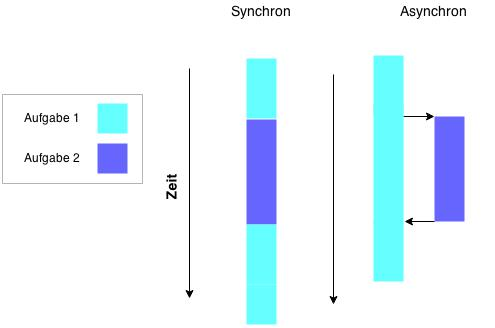
\includegraphics[width=5cm]{images/synchron_vs_asynchron.jpg}
  \caption{
    Synchron vs. Asynchron
  }
  \label{figure:syncron_vs_async}
\end{figure}

Abbildung \ref{figure:syncron_vs_async} zeigt den unterschied zwischen synchron und asynchron. 

\subsection{Blocking vs Non-Blocking}

Unter einer blockierenden Prozedur verstehn man eine Prozedur welche den Aufrufer so lange blockiert bis diese abgeschlossen ist. Generell besitzt jeder Aufruf einer Prozedur in einem linearen Programmierfluss einen blockierenden Charakter. Der Aufrufer einer Funktion wartet so lange bis die Funktion wieder zum Aufrufer zurückkehrt. 

Unter einem nicht blockierenden oder non-blocking Prozedur versteht man eine Prozedur die nicht auf den Abschluss einer Operation wartet sondern sofort zum Aufrufer zurückspringt. Dabei werden mehrere Aufgaben gleichzeitig behandelt.  

In vielen Fällen wird eine blockierende Funktion im Zusammenhang mit I/O Operation gebracht, da diese Operationen nicht an die CPU eines Prozesses gebunden sind. Angenommen eine Prozedur soll eine Datei von der Festplatte einlesen. Die Prozedur fordert dazu das Betriebssystem auf die Datei einzulesen. Dabei kann die Datei entweder blockierend oder nicht blockierend eingelesen werden. Wird die blockierende Variante gewählt so wird die Prozedur so lange pausiert bis die Datei vollständig eingelesen wurde. Wird die nicht blockierende Variante gewählt so fordert die Prozedur das Betriebssystem auf die Datei zu lesen. Während das Betriebssystem die Datei noch einliest wird die Prozedur fortgesetzt. Die Prozedur ist selbst verantwortlich wie sie Zugriff auf die Daten erhält \cite[p. 47]{Erb2012}.

\begin{figure}[!htb]
  \centering
  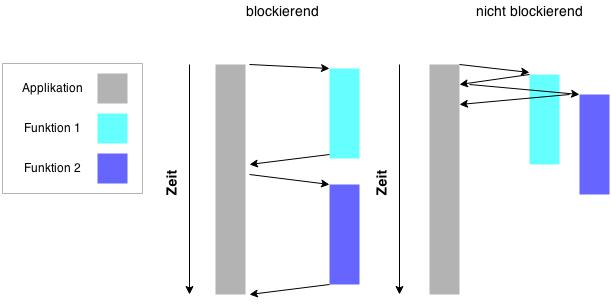
\includegraphics[width=13cm]{images/blocking_vs_nonblocking.jpg}
  \caption{
    Blocking vs Non-Blocking
  }
  \label{figure:blocking_vs_non_blocking}
\end{figure}

Abbildung \ref{figure:blocking_vs_non_blocking} zeigt die unterschiede zwischen blockierenden und nicht blockierenden Prozeduren. Im Bild kann man auch sehen, dass zwei nicht blockierende Prozeduren schneller abgearbeitet werden können und dadurch zu einer gesteigerten Performance führen. 

\subsection{Kombinationen}
Beim blockierenden oder nicht blockierenden Prozeduren geht es grundsätzlich um die Art und Weise wie eine Prozedur auf dem Rechner ausgeführt wird. Bei synchronen oder asynchronen Prozeduren geht es um den Programmierfluss. Kombiniert man die vorher genannten Konzepte so ergeben sich daraus vier unterschiedliche Kombinationen \cite[p. 48]{Erb2012}. 

\subsubsection{Das blockierenden und synchrone Model}
Im blockierenden und synchronen Model werden einzelne Operationen sequentiell abgearbeitet. Wird in diesem Model eine blockierende Operation ausgeführt, wird die Prozedur so lange pausiert bis die blockierende Prozedur abgeschlossen ist. Dannach wird der Programfluss weiter ausgeführt bis die nächste blockierende Operation auftritt oder das Programm terminiert.

Ruft ein Prozess eine blockierende I/O Operation auf so wird der Prozess so lange pausiert, bis das Betriebssystem die Daten vollständig gelesen hat. Durch das blockierende und synchrone Model wird die CPU nicht optimal ausgelastet. In vielen Applikationen spielen I/O Operationen nur eine nebensächliche Rolle. Im Bereich der Webserver sind I/O Operationen jedoch ein wichtiger Bestandteil wodurch dieses Model für den Einsatz bei Webserver nur bedingt geeignet ist \cite[p. 48]{Erb2012}.


\subsubsection{Das nicht blockierende synchrone Model}

Bei diesem Model kehrt eine Prozedur sofort nach dem Aufruf zum AufruferIn zurück. Das Resultat der aufgerufenen Prozedur könnte in diesem Fall noch nicht verfügbar sein. Der Aufrufer selbst muss sich um die synchronisierung der Daten zwischen den beiden Prozeduren kümmern. Dabei muss der Aufrufer selbst den Programmierfluss unterbrechen bis die Prozedur abgeschlossen ist. 

Das nicht blockierende synchrone Model führt zu unnötigen Ressourcenverbauch da die Applikation zwar prinzipiell nicht blockiert, jedoch trotzdem wartet bis eine Operation zu ende ist. Eine Mögliche Implementierung wäre eine Schleife zu verwenden welche abbricht, wenn die Operation abgeschlossen ist.\cite[p. 48]{Erb2012}

\subsubsection{Das blockierende asynchrone Model}

Das blockierende asynchrone Model verwendet einen zweiten Programmierfluss für die Applikation. Durch den blockierenden Charakter verhält sich das blockierende asynchrone Model ähnlich dem blockierenden synchronen Model. 

\subsubsection{Das nicht blockierende asynchrone Model}
Beim nicht blockierenden asynchronen Model kehrt eine blockierende Operation sofort an die aufrufende Funktion zurück. Ist die Operation abgeschlossen wird entweder ein Ereignis getriggert oder eine Callback Funktion ausgeführt. Durch das nicht blockierende asynchrone Model wird die I/O Operation direkt im Kernel des Betriebssystems abgearbeitet. Dadurch kann die Applikation die Zeit in der die I/O Operation ausgeführt wird für andere Aufgaben nutzen \cite[p. 48]{Erb2012}.

Ein Grund warum das asynchrone nicht blockierende Model schneller sein kann als die beiden synchronen Modelle sind I/O Operationen die den Prozess blockieren\ref{subsection: io_operationen}. Angenommen eine Applikation möchte 2 Aufgaben erledigen bei der die erste Aufgabe eine Datei vom Dateisystem einliest. Im Falle der beiden synchronen Modelle müssten die Aufgabe 1 auf das fertige Einlesen der Datei warten. Dies kann entweder auf Kernelebene Funktionieren (= synchrones blockierendes Model) oder auf Applikationsebene (= synchrones nicht blockierendes Model) passieren \cite[]{Pet2015}. 

Im asynchronen nicht blockierenden Model kann die Applikation die Aufgabe 1 ausführen bis die Operation blockiert. Während der Kernel die Datei einliest kann die Applikation die Aufgabe 2 ausführen und nach dem terminieren der Aufgabe 2 wird die Aufgabe 1 abgeschlossen. Dadurch macht das Program immer eine fortschritt ohne dass es auf auf Daten vom Kernel warten muss \cite[]{Pet2015}.

\begin{figure}[!htb]
  \centering
  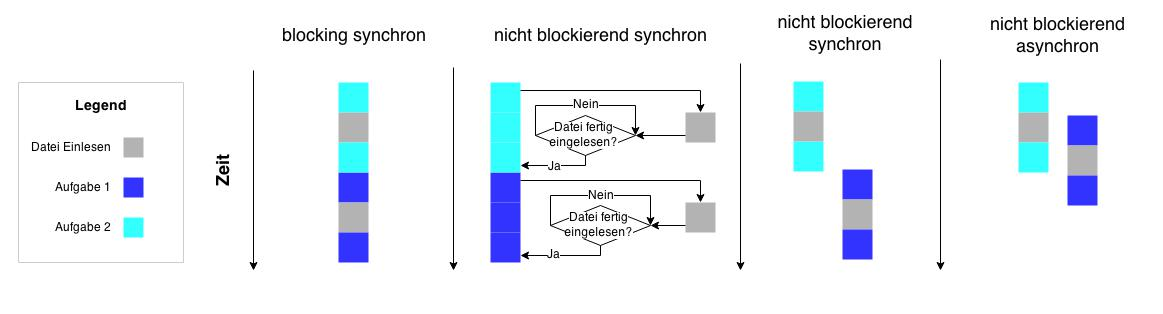
\includegraphics[width=16cm]{images/synchron_blocking.jpg}
  \caption{
    Unterschiedliche Kombinationen im Überblick
  }
  \label{figure:synchron_blocking}
\end{figure}

\subsection{Zusammenfassung}

In diesem Kapitel wurde das Prinzip der asynchronen Programmierung besprochen. Im Bezug auf asynchrone Programmierung kann man Programme in vier unterschiedliche Kategorien einteilen: 

\begin{itemize}
  \item blockierend und synchron
  \item nicht blockierend und synchron
  \item blockierend und asynchron
  \item nicht blockierend und asynchron
\end{itemize}    

Viele Anwendungen welche nur wenige I/O Operationen besitzen verwenden das blockierende und synchrone Model da es einen sequentiellen Programmierfluss erlaubt. Das nicht blockierende und synchrone Model verlagert das Warten auf I/O Operationen vom Betriebssystem in die Applikation, was zu einem unnötigen Ressourcenverbauch führen kann. Das asynchrone und nicht blockierende Model bietet die Möglichkeit die CPU bestmöglich auszunutzen da die Applikation während der I/O Operation eine andere Aufgabe ausführen kann.
\section{Threads}
\label{section: Threads}


(TODO: maybe cover those topics:)
%https://www.wikiwand.com/en/Parallel_Virtual_Machine
%https://www.wikiwand.com/de/Message_Passing_Interface
%http://www.open-mpi.org/



Prozess ist eine squentielle folge von Operationen welche keinen Speicher mit anderen Operationen teilen. (TODO: add to own subheading - maybe to introduction)


(TODO: was ist eine operation was ist ein prozess)

Threads sind Prozesse die sequentiell abgearbeitet werden jedoch den selben Speicher verwenden. \cite[p. 2]{Lee06} Es gibt Applikationen welche Threads








\subsection{Probleme bei verwendung von Multithreading}

\subsection{Race Conditions}

\subsection{Deadlocks}

\subsubsection{The Dining Philosophers Problem}

Edsger Dijkstra beschreibt in seiner Thesis ``Hierarchical ordering of sequential processes'' das Problem des Deadlocks. Dabei beschreibt er folgendes problem:

\begin{quote}
	Five pholosophers numberd 0 through 4 are living in a house where the table laid for them, each philosopher has his own place hat the table. Their only problem - besides those of philosophy - is that the dish served is very difficult kind of spaghetti, that has to be eaten with two forks. There are two forks next to each plate, so that presents no difficulty: as a consequence, however, no two neighbours may be eating simultaniously. \cite[p. 21]{dij71}
\end{quote} 

Alle Philosophen sind mit ihren Gedanken so beschäftigt, dass sie nicht miteinander kommunizieren können. Damit einer der Philosophen essen kann benötigt er beide Gabeln. Eine mögliche Reihenfolge der Operationen die nötig sind damit ein Philosoph essen kann lauten wie folgt \cite[p. 21]{dij71}:

\begin{itemize}
  \item Denke nach
  \item Ist der Philosoph nicht hungrig? Gehe zu Schritt 1
  \item Ist die rechte Gabel nicht frei, Gehe zu Schritt 1
  \item Nimm die rechte Gabel
  \item Ist die linke Gabel nicht frei, Denke Nach und wiederhole diesen Schritt
  \item Nimm die linke Gabel
  \item Esse
  \item Lege rechte Gabel auf den Tisch  
  \item Lege linke Gabel auf den Tisch
  \item Gehe zu Schritt 1
\end{itemize}

Das Problem bei dieser Implementierung ist die Möglichkeit eines Deadlocks. Dieses kann entstehen wenn alle Philosophen zur gleichen Zeit hungrig werden und die jeweils rechte Gabel in die Hand nehmen. Nachdem die jeweils linke Gabel vom rechten Philosophen bereits besetzt ist, denken alle Philosophen so lange nach bis die rechte Gabel frei wird. In diesem Zustand wird keiner der Philosophen jemals satt werden \cite[p. 21]{dij71}. 

Das \emph{Dining Philosophers Problem} kann auf die Informatik angewendet werden bei dem mehrere parallel laufende Threads auf einen geteilten Speicher warten der vom jeweilig anderen Thread blockiert wird. 




\subsection{Context Switching}



\url{https://wiki.haskell.org/Parallelism_vs._Concurrency}

Green Threads vs System Threads

Deadlocks
	\subsection{Threads in Ruby}
\label{section: Threads in Ruby}
\section{Single Threaded Solutions}
\label{section: Single Threaded Solutions}

In diesem Kapitel werden unterschiedliche Design Konzepte vorgestellt wie in modernen Scriptsprachen Concurrency implementiert werden kann, welche auf einem einzelnen CPU Core ausgeführt werden.
	\subsection{Reactor Pattern}
\label{section:Reactor Pattern}

Das Reactor Pattern ist ein Design Pattern bei dem asynchrone auftretende Events, synchron abgearbeitet werden. Asynchrone Nachrichten/Events werden vom Reactor Pattern in einen synchronen Programmfluss gebracht. Neben dem Empfangen von asynchronen Nachrichten kann das Reactor Pattern verwendet werden um nicht blockierende I/O lastige Applikationen zu entwicklen. Da die Registrierung und der Aufruf von Ereignissen vom Reactor Pattern übernommen wird gibt es eine lose Koppelung zwischen dem lesenden und schreibenden I/O Operationen und der Business Logik. \cite[p. 1]{Sch95}

\subsubsection{Motivation}
\label{section:reactor_motivation}

Douglas C. Schmidt beschreibt einen Anwendungsfall für das Reactor Pattern, bei dem Logging Informationen in einem verteilten System an einen zentralen Server gesendet und dort gespeichert werden. Der Server soll in der Lage sein Logging Informationen zu jederzeit speichern zu können. Dabei kann es vorkommen, dass Informationen auch von mehreren Clients gleichzeitig an den Server gesendet werden \cite[p. 1]{Sch95}. 

Eine Möglichkeit um mehrere Verbindungen auf einmal zu verarbeiten bietet Multithreading. Laut D. Schmidt können bei der Verwendung von Multithreading folgende Probleme auftreten \cite[p. 1]{Sch95}: 

\begin{itemize}
  \item benötigt ein komplexes concurrency Schema
  \item auf Single Core Prozessoren kann es zu einer schlechten Performance kommen
  \item es könnte nicht auf allen Betriebssystemen verfügbar sein.
\end{itemize}

Die Nachteile 2 und 3 können 20 Jahre nach dem Erscheinen dieses Papers als hinfällig angesehen werden, da mittlerweile multicore Prozessoren im Consumer Bereich angekommen sind und jedes relevante Betriebssystem Threads unterstützt. Das Problem Nummer 1 mit dem komplexen concurrency Schema bei der Verwendung von Multithreading bleibt bis heute bestehen. Das Reactor Pattern wurde 1995 entwickelt und probiert alle drei dieser Probleme zu lösen indem es auf Multithreading verzichtet.

\subsubsection{Funktionsweise}

Das Reactor Pattern implementiert eine Event Loop, welche sich um das Versenden und Empfangen von Events kümmert. Die Event Loop ist eine nicht endende Schleife, die Events von außerhalb empfangen kann und dieser an den richtigen Empfänger weiterleitet. Um auf einen Ereignistyp reagieren zu können verwendet das Reactor Pattern Callback Funktionen, welche aufgerufen werden sobald ein Ereignis eintritt. Dadurch kann eine Applikation nur auf Ereignisse reagieren, für welche eine Callback Funktion verfügbar ist. Da das Reactor Pattern auf Multithreading verzichtet, kann immer nur eine Operation zu einem Zeitpunkt ausgeführt werden. I/O Operationen können jedoch gleichzeitig behandelt werden. In der Regel werden Callback Funktionen ausgeführt, wenn eine blockierende I/O Operation abgeschlossen ist. Folgende typische Ereignisse können im Reactor Pattern auftreten \footnote{Die Liste ist angelehnt an folgenden Blog-Post: \url{http://pltconfusion.com/2014/10/20/eventmachine_internals_and_the_reactor_pattern/}}:

\begin{itemize}
  \item eine Datei wurde von einem Filesystem gelesen
  \item eine Datebankabfrage wurde gelesen
  \item ein HTTP Request wurde komplettiert
\end{itemize}

Ob eine I/O Operation bereits abgeschlossen ist und dadurch nicht blockiert, kann zum Beispiel über den Systemaufruf \emph{select} \footnote{Siehe auch Sektion \ref{section: Threads} Threads} bestimmt werden.

Der genaue Lebenszyklus des Reactor Patterns ist in Abbildung \ref{figure:reactor_cycle} beschrieben.

\begin{figure}[!htb]
  \centering
  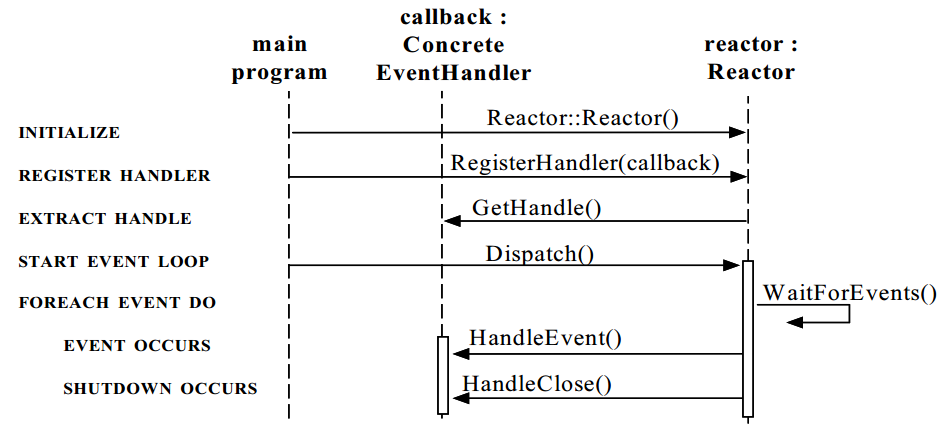
\includegraphics[width=13cm]{images/reactor.png}
  \caption{
    Zusammenarbeit der einzelnen Komponenten \cite[p. 5]{Sch95}
  }
  \label{figure:reactor_cycle}
\end{figure}

In der Initialisierung wird der Reactor in der \emph{main} Methode erstellt. Nachdem ein Reactor erstellt wurde, können sich unterschiedliche \emph{Event Handler} beim Reactor registrieren. Ein \emph{Event Handler} ist eine Klasse, die auf ein bestimmtes Ereignis reagieren kann. Diese \emph{EventHandler} besitzt eine \emph{getHandler} Methode, welches die Callback Methode für ein Ereignis zurückliefert. Sind alle Handler beim Reactor registriert startet die Eventloop und wartet auf Ereignisse. Sobald ein Event eintritt wird die Callback Methode ausgeführt. Im letzten Schritt wird der Handler geschlossen und die Eventloop wartet auf die nächsten Ereignisse. 

Wie genau die Eventloop einzelne Ereignisse behandelt, variiert zwischen den einzelnen Implementierungen. Eine mögliche Implementierung ist das Ereignis an das Ende einer Queue zu geben und bei jedem Durchlauf der Eventloop wird genau ein Ergebnis von der Queue genommen und behandelt.

Der Ablauf, der in Abbildung \ref{figure:reactor_cycle} beschrieben ist richtet sich sehr an statische Programmiersprachen wie C++\footnote{In Kapitel \ref{section:implementation} wird das Reactor Pattern in Ruby Implementiert.}.

Durch die Verwendung des Reactor Patterns wird eine enge Koppelung zwischen unabhängigen Teilen der Applikation und Applikations abhängigen teilen gelöst. Dadurch werden die Tief liegenden und komplexen Komponenten wie das Empfangen und Versenden von Events, von der EventLoop übernommen \cite[p. 2]{Sch95}.

\subsubsection{Reactor - Design Pattern}

In Abbildung \ref{figure:reactor_otm} wird die OTM Notation verwendet \footnote[0]{OTM ist der vorgänger von UML nähere Informationen findet man unter: \url{http://www.uml.org/}}.

\begin{figure}[!htb]
  \centering
  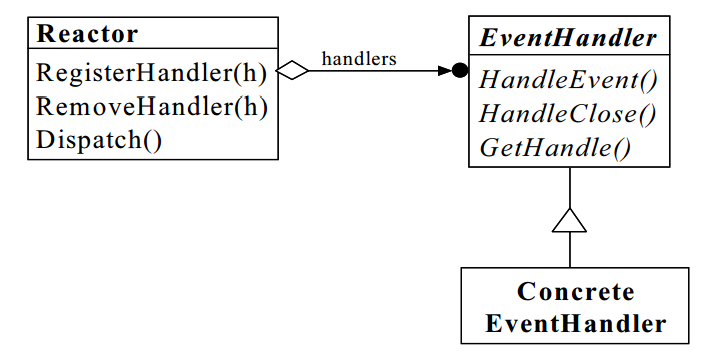
\includegraphics[width=9cm]{images/reactor_otm.png}
  \caption{
    Reactor OTM \cite[p. 4]{Sch95}
  }
  \label{figure:reactor_otm}
\end{figure}

\cite[p. 2]{Sch95}

\emph{Reactor:}
 Die Reactor Klasse ist für das Registrieren, Entfernen und Versenden von Ereignissen verantwortlich. Die Eventloop, welche Callback Methoden von Ereignissen ausführt, befindet sich ebenfalls in dieser Klasse. Der Reactor ist unabhängig von der Applikation und kann deswegen in anderen Applikationen wiederverwendet werden. 

\emph{Event Handler:}
Die Eventhandler Klasse bietet ein Interface für einen konkreten EventHandler. In dynamischen Sprachen wie Ruby oder JavaScript, die keine Interfaces bieten ist diese Klasse hinfällig. 

\emph{ConcreteEventHandler:}
Der ConcreteEventHandler implementiert das Interface des Event Handlers. Dabei muss der Eventhandler folgende drei Methoden beinhalten: GetHandle, HandleEvent und StopEvent.

\subsubsection{Anwendungsgebiete}

Douglas Schmidt beschreibt in seiner Thesis folgende Anwendungsgebiete für das Reactor Pattern \cite[p. 4]{Sch95}:

\begin{itemize}
  \item Ein oder mehrere Ereignisse können gleichzeitig von unterschiedlichen Clients kommen
  \item Das Blockieren eines Clients oder das Pollen von Requests ist zu ineffizient
  \item Die gesendeten Nachrichten können in relativ kurzer Zeit verarbeitet werden
  \item Wenn unabhängige Teile der Applikation (Event Demultiplexing/Dispatching) von den abhängigen Teilen der Applikation getrennt werden sollen
\end{itemize}

\subsubsection{Zusammenfassung}

Das Reactor Pattern bietet die Möglichkeit asynchron auftretende Ereignisse synchron zu verarbeiten. Durch den bewussten Verzicht auf Multithreading werden Probleme wie Deadlocks oder Race Conditions verhindert. Um dennoch mehrere Ereignisse gleichzeitig bearbeiten zu können, verwendet das Reactor Pattern eine bis zum Ende des Prozesses laufende Schleife. Diese Event Loop kümmert sich um das Empfangen und Versenden von Ereignissen. Dadurch werden asynchron auftretende Ereignisse wie sie bei einem Webserver auftreten können in einen synchronen Kontrollfluss gebracht. 

Das Reactor Pattern findet seine Einsatz in Applikationen welche durch viele blockierende I/O Operation abhängig sind. Durch die Verwendung des Reactor Patterns wird der Prozess nicht blockiert und somit in keinen Ruhezustand versetzt.
	\subsection{Proactor vs. Reactor Pattern}
\label{section: Proactor vs. Reactor Pattern}
\section{Multi Threaded Solutions}
\label{section: Multi Threaded Solutions}

Multi Threaded Applikationen benutzen mehrere Threads in einer einzelnen Applikation. \cite[p. 1]{DabMIT}


(TODO: write about Moore’s Law)

\subsection{Multithreading Pitfalls}
\label{subsection: multithreading pitfalls}

\cite[p. 2]{Sch97}



	\subsection{Proactor Pattern}
\label{section: Proactor Pattern}

Das Proactor Pattern ist ein Designpattern um asynchrone Events durch einem Pool von einem oder mehreren Threads zu bearbeiten. Durch das verwenden von Threads kann das Proactor Pattern Anfragen parallel verarbeiten. 

\subsubsection{Motivation}
Das Proactor Pattern kann als eine Erweiterung des Reaktor Pattern verstanden werden. Der unterschied zwischen Proactor und Reactor ist dass das Reactor Pattern die I/O Operationen im eigenen Thread ausführt und das Proactor Pattern die I/O Operationen an das Betriebssystem weiterleitet. Dabei wartet das Proactor Pattern auf Callback Funktionen und das Reactor Pattern wartet auf Events. \cite[p. 7]{CZY2009}

Das Proactor Pattern findes seine Anwendung in Applikationen welche davon profitieren asynchrone Operationen gleichzeitig auszuführen. Durch das Reactor Pattern können Applikationen entwickelt werden welche keine Rücksicht auf die Beschränkungen (TODO: write about constraints of reactive/multithreaded programming) von Multithreaded Programming nehmen. (Die Einschränkungen von Multithreading werden in \ref{subsection: multithreading pitfalls} näher erläutert.) \cite[p. 1]{Sch97}

\subsubsection{Funktionsweise}

Der Initialisierungsvorgang:

(TODO: write about initialisation)
\cite[p. 3]{Sch97})


Die Funktionsweise eines Webservers welcher mit dem Proaktor Patterns implementiert ist wird in 8 Schritten unterteilt: 
(TODO: Add Image from \cite[p. 4]{Sch97})

1: Der Client sendet einen HTTP GET Request (z.B. index.html)(TODO: ask Hannes if should i write about HTTP GET Requests) an den Webserver.  

2: Das Betriebssystem beendet den Lesevorgang des HTTP Requests und ruft die Completion Dispatch Methode auf. 

3: Der Completion Dispatcher benachrichtigt den HTTP Handler, dass es einen neuen HTTP Get Request gibt. 

4: Der HTTP Handler analysiert den HTTP Request.

5: Der HTTP Handler liest die Datei index.html synchron vom Dateisystem ein.

6: Der HTTP Handler initialisiert eine asynchrone Operation um die Datei in die Client Connection zu schreiben. Dabei gibt er sich selbst als Completion Handler an. Weiters referenziert der HTTP Handler den Completion Dispatcher, welcher benachrichtigt wird, wenn die Datei an den Client geschrieben worden ist. 

7: Wenn der Schreibvorgang abgeschlossen ist wird der Completion Dispatcher benachrichtigt. 

8: Der Completion Dispatcher benachrichtigt den Completion Handler. 


\subsubsection{Anwendungsgebiete}

Doughlas C. Schmidt et al. beschreibt folgende Anwendungesgebiete für das Proaktor Pattern \cite[p. 5]{Sch97}):

\begin{itemize}
  \item Die Applikation muss eine oder mehrere asynchrone Operationen ausführen ohne den Thread zu Blockieren.
  \item Die Applikation muss benachrichtigt werden wenn eine asynchrone Operation beendet ist. 
  \item Die Applikation profitiert von einer losen Koppelung zwischen der abhängigen und unabhängigen Logik der Applikation
  \item Die Applikation ist mit Multithreading oder dem Reactor Pattern implementiert und liefert eine schlechte Performance. 
\end{itemize}

\subsubsection{Struktur des Patterns}

(TODO: add image \cite[Figure 8]{Sch97}))

\emph{Proactive Initiators initiates operation}
	Der Proaktiv Initiator registriert die asynchronous operation processor, den Completion Dispatcher und den Completion Handler. 

\emph{Asynchronous Operation Processor}




Im folgenden wird das Proactor Design Pattern in der OTM Notation vorgestellt. \footnote[0]{Mehr Informationen zur OTM Notation: \url{http://www.uml.org/}}

(TODO: add image \cite[Figure 7]{Sch97}))

\emph{Proactor Initiator}
	Der Proactor Initiator ist der Teil des Proactor Patterns welcher asynchrone Operationen initialisiert. Der Initiator erstellt den \emph{Completion Dispatcher}, welcher ein asynchrone Operation beinhaltet. Des weiteren erstellt er 

	\subsection{Actor Based Model}
\label{section:Actor Based Model}

Das Actor Based Model ist ein Model um Concurrent Applikation zu entwickeln, bei dem das Problem des Shared States durch das versenden und erhalten von Nachrichten behoben wird. 

\subsubsection{Einführung}

Das Actor Based Model basiert auf den drei Grundlegenden Elementen der Informatik:

\begin{itemize}
  \item Processing (Daten müssen verarbeitet, geändert werden)
  \item Store (Daten müssen verarbeitet weren)
  \item Communication
\end{itemize}

Dabei sind Actors Zeitsensitiv, was bedeutet, dass sie Ihren Status über eine gewisse Zeit ändern können. Jeder Actor besitzt eine Mailbox und bei jeder neu erhaltenen Nachricht gibt es drei Möglichkeiten wie er auf diese reagieren kann:

\begin{itemize}
  \item Er kann neue Actoren erstellen
  \item Er kann Nachrichten an andere Actoren senden
  \item Er kann bestimmen wie er die nächste Nachricht verarbeiten möchte
\end{itemize}

Um Nachrichten versenden zu können, benötigen Actoren eine Adresse. Dabei ist eine Adresse keine Identität eines Actors, da ein Actor keine, eine oder mehrere Adressen besitzen kann. Um anderen Actoren eine Nachricht zu senden muss der Sender die Adresse des Empfängers wissen. Dabei kann der Sender der selbe Actor sein wie der Empfänger. Das bedeutet, dass sich ein Actor selbst Nachrichten senden kann und diese in der Zukunft verarbeitet werden. Dabei darf Actors keinen geteilten Status mit einem anderen Actor besitzten. Dadurch dürfen nur unveränderbare Daten (ummutable Data) von einem Actor zum anderen versendet werden. Pointer und Referenzen dürfen deshalb kein Teil der Nachricht sein. \cite[]{Erb2012}

Nachrichten werden asynchron versendet und können beliebig lange für die Zustellung benötigen. Es wird keine Garantie über die Reihenfolge gegeben in der Nachrichten beim Empfänger ankommen. Es gibt jedoch Implementierungen des Actor Based Models, welche die Reihenfolge der versandten Nachrichten beibehält. Um Race Conditions zu vermeiden müssen alle Nachrichten unveränderbar sein. Dies kann mit dem Begriff `Call by Value' verglichen werden, bei dem eine Variable bei einem Funktionsaufruf kopiert wird. Dadurch können keine Race Conditions auftreten da jeder Actor seine Mailbox squentiell abarbeitet und kein Speicher mit anderen Objekten teilt. Dadurch sind einzelne Actoren in einem System aus Actoren unabhängig da die Kommunikation nur über Nachrichten passiert. \cite[]{Erb2012}

Das Actor Based Model bestimmt nicht in welcher Art und Weise die Kommunikation zwischen den einzelnen Actoren passiert, da dies der jeweiligen Implementierung vorenthalten ist. Dadurch kann geschlossen werden, dass das Actor Based Model auch in verteilten Systemen zum Einsatz kommen kann \cite[]{Erb2012}.

Actors haben einen isolierten Zustand, welcher von keinem anderen Actor verändert werden kann. Dadurch benötigen viele Implementierungen keine Locks für geteilte Daten, weil nur unveränderbare Objekte verteilt werden können. 

Dadurch das ein Actoren nur über Nachrichten miteinander kommunizieren können und die Reihenfolge und Zeit in der Nachrichten übermittelt werden nicht bestimmt ist, ist das Actor Based System nicht deterministisch \cite[]{Agh85}. Wenn ein Algorithmus nicht deterministisch ist bedeutet das, dass bei den exakt selben Eingabewerten bei mehreren durchgängen andere Resultate auftreten.

Ein Beispiel für einen nicht deterministischen Algorithmus in einem Actor Based Model wäre das einfach inkrementieren einer Zahl. Dazu nehmen wir an dass es einen Actor A gibt der die Variable x mit dem Wert 0 besitzt. Dieser soll sich selbst so lange die Nachricht `Inkrement 1' schicken. Erhält er die Nachricht `Show Value' soll er den aktuellen Wert auf der Konsole ausgeben.

Zu Begin bekommt er von einem entfernten Actor B die Nachricht `Start Inkrement'. Daraufhin schickt er sich selbst die Nachricht `Inkrement 1'. Beim erhalten der Nachricht wir diese in die Mailbox gepackt und abgearbeitet. Beim abarbeiten der Mailbox wird die lokale Variable x um 1 erhöht und besitzt somit den Wert 1. Nachdem der Wert erhöht wurde versendet der Actor A eine weitere Nachricht mit dem Inhalt `Inkrement 1' an sich selbst. Zum exact selben Zeitpunkt versendet der Actor B die Nachricht `Show Value'. Nachdem das Actor basierte Model die Reihenfolge der Nachrichten nicht behandelt kann die Nachricht `Show Value' entweder vor oder nach der Nachricht `Inkrement 1' ankommen. Kommt die Nachricht `Show Value' vor der Nachricht `Inkrement 1' an so wird der Wert 1 in der Konsole ausgegeben. Anderenfalls wird der Wert 2 ausgegeben.

\subsection{Probleme}
Auch wenn das Actor Based Model Probleme von paralleler Programmierung verhindern kann, können dennoch Deadlocks auftreten. So kann eine zyklische Abhängigkeit entstehen, wenn zwei Actoren jeweils auf eine Nachricht des anderen warten. In der Praxis kann jedoch ein Deadlock in einem Actor Based Model durch ein Timeout behoben werden. Durch die asynchrone Funktionsweise können nicht deterministische Algorithmen entstehen, welche bei falsche implementierung als eine Race Condition angesehen werden können \cite[]{Erb2012}. 

\subsection{Implementierungen}
Das Actor Based Model kann entweder Sprachkonzept direkt in eine Programmiersprache eingebaut werden oder als Bibliothek zu einer bestehenden Programmiersprache hinzugefügt werden. Die folgende Liste gibt einen Aufschluss über Programmiersprachen welche das Actor Based Model direkt in die Programmiersprache integriert haben \footnote{Eine erweiterte Liste findet sich auf: \url{http://en.wikipedia.org/wiki/Actor_model?oldformat=true#Programming_with_Actors}}:

\begin{itemize}
  \item Erlang
  \item Elixir
  \item Rust
  \item D
  \item E
\end{itemize}

Die folgende Liste gibt einen Überblick über einzelne Bibliotheken welche das Actor Based Model anbieten:

\begin{itemize}
  \item celluloid (ruby \url{https://celluloid.io/})
  \item nactor (JavaScript \url{https://github.com/mental/webactors})
  \item akka (Java und Scale \url{http://akka.io/})
  \item Pykka (Python \url{https://www.pykka.org})
\end{itemize}

Die beiden vorherigen Listen erheben keinen Anspruch auf Vollständigkeit. 

\subsubsection{Zusammenfassung}
Das Actor Based Model ist ein Model welches auf drei Grundlegenden Komponenten der Informatik basiert (Datenverarbeitung, Datenspeicherung, Kommunikation). Dabei Kommunizieren Actors über Nachrichten miteinander, welche in der Mailbox des Empfängers ankommen und sequentiell abgearbeitet werden. Das Actor Based Model bestimmt nicht in welcher Art und Weise die Nachrichten übertragen werden. Das bedeutet das je nach Implementierung die Reihenfolge in welcher Nachrichten beim Empfänger ankommen nicht bestimmt ist. 

Es gibt drei Möglichkeiten wie ein Actor eine Nachricht verarbeiten kann (Neue Actoren erstellen, Er kann eine Nachricht an andere Versenden, Er kann bestimmen wie er die nächste Nachricht verarbeiten möchte).

Um Race Conditionen zu vermeiden dürfen Nachrichten nur aus unveränderbaren Daten bestehen. Das übermitteln von Referenzen oder Pointer zu anderen Actoren ist verboten. Dadurch entsteht eine innere Kapselung der Daten eines einzelnen Actors was dazu führt, dass sich das Actor Based Model für parallele Programmierung anbietet. Es können zwar Deadlocks oder Race Conditions entstehen wobei diese Hauptsächlich als Fehler in der Applikation gesehen werden können. 


\section{Ruby}
\label{section: Ruby}

In diesem Kapitel wird die Programmiersprache Ruby kurz vorgestellt. Dieses Kapitel ist nicht mit einer Einführung in Ruby vergleichbar, da eine solche über den Rahmen dieser Arbeit hinausgehen würde. Das Buch Programming Ruby \cite[]{Dav05} bietet eine Einführung in die Sprache kann als Referenz dienen. 

Auf der Website \footnote{\url{http://www.ruby-lang.org}} definiert sich Ruby wie folgt:

\begin{quote}
	Ruby ist eine dynamische, freie Programmiersprache, die sich einfach anwenden und produktiv einsetzen lässt. Sie hat eine elegante Syntax, die man leicht lesen und schreiben kann. \cite[]{Rub92}
\end{quote}

Im Kern ist Ruby eine rein Objekt Orientierte Programmiersprache. Dabei besteht ein Objekt aus einer Kombination von Status und Methoden welche diesen Status verändern. \cite[p. 1-2]{Dav05}

Ruby wurde im Jahr 2012 von der ISO (International Organization for Standardization) mit dem Standard ISO/IEC 30170 \footnote{Den Standard kann man der Website \url{http://www.iso.org/iso/home/store/catalogue_tc/catalogue_detail.htm?csnumber=59579} erwerben} standardisiert. Die Referenzimplementierung von Ruby ist CRuby oder MRI (Matz's Ruby Interpreter) \footnote{Der Quellcode ist auf Github verfügbar: \url{https://github.com/ruby/ruby}}.


\subsection{Concurrency in Ruby}

\subsubsection{Threads in Ruby}
In Ruby wird jedes Program in einem Thread ausgeführt. Dieser Main Thread wird beim ausführen eines Ruby Programms automatisch erstellt und ausgeführt. Wird der Main Thread beendet, so werden gleichzeitig alle anderen Threads der Applikation beendet und der Ruby Prozess wird beendet \cite[p. 15]{Sto2013}.

Um einen Thread in Ruby zu erzeugen erstellt man ein neues Thread Objekt und übergibt diesen einen Block. 

\begin{lstlisting}[language=Ruby,label=lst:thread_example]
def long_running
	sleep 2
	puts "second"
end
Thread.new { long_running }
puts "first"

# Output
#
# => first
# => second

\end{lstlisting}

In Listing \ref{lst:thread_example} sieht man ein Ruby Script welches einen Thread verwendet. Durch die Methode \emph{sleep} wird die Methode \textit{long\_run\_running} zwei Sekunden gestoppt. Im Beispiel sieht man dass die Zeile 6 als erstes auf dem Monitor ausgegeben wird als die Zeile 3. 

\cite[p. 21]{Sto2013}
\begin{lstlisting}[language=Ruby]
  100.times do
    Thread.new { sleep }
  end
  
  puts  "ps -o nlwp #{Process.pid}"
  sleep
\end{lstlisting} 

Dieses Programm erstellt 100 Threads und versetzt diese in einen schlafenden Zustand. Nachdem all Threads erstellt wurden wird der Main Thread in einen schlafenden Zustand versetzt. Daraus Resultiert, dass dieses Programm 101 Threads verwendet. 

Vergleicht man die unterschiedlichen Implementierungen von Ruby so kann man erkennen dass MRI, Rubinius, und JRuby weitere Threads zum verwalten von Ruby verwenden. MRI verwendet 1 zusätzlichen Thread zum verwalten. Bei JRuby und Rubinius richtet sich die Anzahl an Threads zum verwalten von Ruby an die verwendete CPU.

\subsubsection{Thread-Safety in Ruby}
In MRI (seit Version 1.9), Rubinius und JRuby werden Native Threads des Betriebssystems verwendet. Dadurch verwenden diese Implementierungen den Scheduler des Betriebssystems. Aus diesem Grund hat die Ruby Implementierung keinen Einfluss auf den genauen Zeitpunkt der Context-Switches. Dadurch können Race Conditions entstehen, welche für falsche Daten verantwortlich sind.

Der Conditional Assignment Operator in Ruby (||=) wird häufig verwendet um einer Variable einen Standardwert zu zuweisen. Dabei ist dieser Operator nicht Thread-Safe, da er keine Atomare Operation darstellt. Hinter diesem Operator steht eine Funktion welche wie folgt aussehen könnte \footnote{Die genaue Implementierung dieses Operators kann sich zwischen den einzelnen Ruby Implementierungen unterscheiden. Das Funktionsweise ist bei allen Implementierungen gleich}:

,caption={\cite[p. 24]{Sto2013}}

\begin{lstlisting}[language=Ruby,label={listing:conditional}]
	\# Dieser Ausdruck
	@results ||= "test" 

	\# Ist gleich diesem Ausdruck
	unless @results.defined?
		@results = "test"
	end
\end{lstlisting} 

In dem Listing \ref{listing:conditional} kann man erkennen das der Conditional Assignment Operator keine atomare Operation ist. Angenommen ein Programm möchte 10 Bilder aus dem Internet downloaden:

(TODO: Continue to Write on this section)

\subsubsection{The GIL in MRI}

Der GIL (Global Interpeter Lock) ist ein globaler Lock um der das parallele Ausführen von Ruby Code in einem Ruby Prozess verhindert. Das bedeutet, dass immer nur ein Ruby Thread pro Prozess einen Fortschritt machen kann. Wenn ein Thread einen fortschritt machen möchte muss er den GIL erhalten und darf nur dann einen fortschritt machen. Das bedeutet nicht dass in Ruby keine concurrent Applikationen geschrieben werden können, denn sobald ein Thread auf eine blockierende Operation trifft (z.B. I/O) dann wird der GIL an einen anderen Thread vergeben. Zu einem späteren Zeitpunkt erhält der blockierte Thread den GIL wieder und kann die Daten weiterverarbeiten. Das bedeutet jedoch das in MRI Ruby Code nie parallel laufen kann \cite[p. 42]{Sto2013}. 

Die Funktionsweise des MRI kann man anhand der Berechnung der Fibonacci Zahl \footnote{Weiter Informationen zur Fibonacci Zahlenfolge finden Sie auf \url{http://de.wikipedia.org/wiki/Fibonacci-Folge}} erklären. Bei diesem Beispiel sollten 4 mal die Fibonacci Zahlen bis 35 berechnet werden:

caption={\cite[p. 21]{Sto2013}}

\begin{lstlisting}[language=Ruby,label={listing:fibonacci}]
class Fibonacci
  def initialize(threads, number)
    @threads = Array.new(threads) { Thread.new {calculate number}}
    @threads.each(&:join)
  end

  #
  def calculate(number)
    return  number  if ( 0..1 ).include? number
    ( calculate( number - 1 ) + calculate( number - 2 ) )
  end
end

Fibonacci.new 4, 35
\end{lstlisting}

In Listing \ref{listing:fibonacci} wird die Fibonacci Zahl 4 mal berechnet. Dazu wird für jede Berechnung ein neuer Thread erstellt. Wird das Programm aus Listing \ref{listing:fibonacci} mit MRI ausgeführt so wird das Program wie folgt ausgeführt \footnote{Es wird nur die Funtionsweise der Zeilen 3-4 Beschrieben} \cite[p. 45-46]{Sto2013}: 

\begin{itemize}
  \item In Zeile 3 wird ein neues Array erstellt, welches mit 4 Threads initialisiert wird \footnote{Die Threads heißen in weiterer Folge Thread 1-4}.
  \item Jedem dieser Threads wird ein Block übergeben in dem die Funktion \emph{calculate} aufgerufen wird. Diese Funktion berechnet die Fibonacci Zahlen bis 35.
  \item Alle 4 Threads möchten einen Fortschritt machen. Jedoch darf nur der Thread einen Fortschritt machen, der den GIL besitzt. Aus diesem Grund werden alle Threads in einen Schlafzustand versetzt.
  \item Der Ruby Interpeter entscheidet, dass der Thread 2 den GIL erhält und weckt den Thread auf.
  \item Der Thread 2 berechnet die Zahlenfolge bis er fertig ist und gibt den GIL zurück an den Ruby Interpreter.
  \item Dieser entscheidet dass Thread 3 den GIL bekommt.
  \item Hat Thread 3 die Berechnung abgeschlossen wiederholt sich die selbe Prozedur für Thread 1 und Thread 4.
  \item Haben alle Threads die Berechnung beendet, ist das Programm abgeschlossen.
\end{itemize}

Der GIL ist eine Beschränkung von Parallelem ausführen von Ruby Code. Rubinius und JRuby heben den GIL auf und können dadurch Code parallel ausführen. Auch wenn der GIL eine große Beschränkung für das parallele Ausführen von Ruby Code darstellt gibt es Gründe warum das Team von MRI am GIL festhalten möchte. Hauptsächlich möchte man das Problem von Race Conditionen vermeiden \cite[p. 48-49]{Sto2013}.

Angenommen man besitzt folgendes Program\footnote{Idee von: \url{http://stackoverflow.com/questions/19969551/why-no-race-condition-in-ruby}}: 

\begin{lstlisting}[language=Ruby,label={listing:race condition}]

class Calculator
  attr_accessor :counter
  def initialize
    @counter = 0
  end
end

calculator = Calculator.new

threads = []
threads << Thread.new {100000.times { calculator.counter += 1 }}
threads << Thread.new {100000.times { calculator.counter += 1 }}
threads.each(&:join)

puts calculator.counter

\end{lstlisting}

In Listing \ref{listing:race condition} werden zwei Threads verwendet um eine Zahl 100000 mal zu erhöhen. Das Resultat der Berechnung sollte \emph{200 000} sein. Wird die Funktion mit MRI ausgeführt erhält man den Wert \emph{200 000}. Wird das Programm mit Rubinius oder JRuby ausgeführt erhält man den Wert \emph{200 000} nicht. 































Die Klasse Thread bietet einige Methoden um mit Threads in Ruby zu arbeiten. \footnote{Eine genaue Dokumentation findet sich unter \url{http://ruby-doc.org/core-2.2.0/Thread.html}}

\subsubsection{Fibers}
Fibers sind leichtgewichtige Objekte in Ruby welche Concurrency ermöglichen. Dabei akzeptieren Fibers Code Blöcke welche von der Applikation gestartet, pausiert und weitergeführt werden können. Im Unterschied zu Threads wird der Zeitplan von Fibers nicht von der Ausführenden Umgebung (Virtuellen Maschine) bestimmt sondern vom Programmierer. 

Jede Fiber besitzt einen eigenen 4kb großen Call-Stack der das Pausieren eines Fibers ermöglicht. Fibers werden nicht automatisch gestartet und müssen manuell vom Programmierer gestartet werden.

\begin{lstlisting}[language=Ruby,label=lst:thread_example]
def long_running
	sleep 2
	puts "second"
end
Thread.new { long_running }
puts "first"

# Output
#
# => first
# => second

\end{lstlisting}



\subsection{Ruby Implementierungen}

Für die Programmiersprache Ruby gibt es unterschiedliche Implementierungen auf welche ich in diesem Kapitel eingehen möchte. Folgende Implementierungen werden in dieser Arbeit nicht behandelt da diese entweder nicht mehr aktiv Weiterentwickelt werden oder für diese Arbeit keine Relevanz besitzten:

\begin{itemize}
  \item MacRuby
  \item MRuby
  \item IronRuby
  \item MegLev
  \item Cardinal
  \item Ruby Enterprise Edition
\end{itemize}

Compiler wie Rubymotion \footnote{Cross Plattform Ruby Compiler für IOS und Android \url{http://www.rubymotion.com/}}, welche Ruby Code in eine andere Programmiersprache kompilieren, werden in dieser Thesis ebenfalls nicht besprochen.

\subsection{CRuby}


\subsection{JRuby}


\subsection{Rubinius}
Rubinius ist eine Implementierung von Ruby welche sich auf Concurrency spezialisiert hat. Dabei verwendet es native Threads um Ruby Code auf allen CPUs laufen zu lassen. Rubinius wird nicht interpretiert sondern besitzt einen JIT (Just In Time) Compiler. Dabei wird der Ruby Code in Bytecode transformiert, welcher von der Ribinius Virtual Maschine ausgeführt wird. Die virtuelle Maschine ist in C und C++ geschrieben und verwendet Teile wie den Ruby Parser von MRI. Die Sprache Ruby ist selbst in Ruby implementiert und kann auf der Virtuellen Maschine ausgeführt werden. Dadurch ist Rubinius eine Implementierung die zu einem großen Teil in Ruby implementiert ist. 


\section{Asynchronous Programming in Rails}
\label{section: Asynchronous Programming in Rails}
	\subsection{Delayed Jobs}
\label{section: Delayed Jobs}

\subsubsection{Queues}
\label{section: Queues}
\section{Zusammenfassung}
Ruby ist eine ausdrucksvolle Programmiersprache, welche grundsetzlich parallele Programmierung erlaubt. Die Referenzimplementierung CRuby kann durch GIL keine Operationen parallel ausführen. Dadurch werden zum einen häufig auftretende Probleme wie Race Conditions und Deadlocks verhindert, jedoch können diese dennoch auftreten. Yukihiro Matsumoto der Erfinder von Ruby hat bei der Rubycon 2012 in Denver auf die Frage nach der Zukunft von Concurrency in Ruby folgende Antwort gegeben:

	``
	I don't consider myself as the threading guy, so I don't think I can make the right decision about the Actor library or the threading library.
	'' (Yukihiro Matsumoto, Rubyconf 2012)

Daraus könnte man schließen dass in Zukunft die Bibliothek Celluloid oder eine andere Bibliothek in die Ruby Standard Library hineinfliesen könnte. Dieses Zitat ist jedoch aus dem Jahr 2012 und bis heute gibt es nur vereinzelt Verbesserungen im Bereich von Concurrency. Es gab bereits Bestrebungen den GIL aus Ruby MRI zu entfernen und ihn mit einzelnen fein dosierten Locks zu ersetzen. Dieser Versuch schlug jedoch fehl da einzelne Locks zu einem Performance verlust bei Applikationen führte, welche nur einen Thread verwenden. 

Abschließend kann man sagen das man mehrere Operationenen in allen Ruby Interpreter gleichzeitig behandeln kann. Threads werden seit langer Zeit eingesetzt und werden von jedem relevanten Betriebssystem unterstützt. Auf dem ersten Blick sieht das verwenden von mehreren Threads relativ einfach aus. Probleme wie Race Conditions und Deadlocks können dabei relativ häufig auftreten und zu korrupten Daten oder einem Absturz der Applikation führen. Um diese Probleme zu lösen können Design Patterns wie das Reactor Patter, Actor Based Model oder Futures helfen. Für Concurrency in Ruby bietet sich das Projekt \emph{Concurrenc Ruby}\footnote{Genaue Informationen zu Concurrent Ruby\url{https://github.com/ruby-concurrency/concurrent-ruby}} an. In diesem Projekt findet sich eine Sammlung an unterschiedlichen Design Patterns und Datenstrukturen welche Thread-Safe sind für die Programmiersprache Ruby.

Ruby ist trotz aller bemühungen eine eher langsame Sprache \footnote{vgl. \url{http://benchmarksgame.alioth.debian.org/u32/compare.php}}. Je nach Interpreter können sich Zahlen bei einzelnen Algorithmen enorm unterscheiden. Aus diesem Grund gibt es Bestrebungen, Applikationen wie den CSS Preprocessor SASS, in einer schnelleren Sprache wie C neu zu implementieren. Für parallelisierbare Algorithmen welche keine oder nur wenige I/O Operationen durchführen empfiehlt es sich deshalb auf MRI zu verzichten und Rubinius oder JRuby zu verwenden. Ist diese Steigerung der Performance noch nicht genug empfiehlt es sich auf andere Sprachen wie Go, Scala oder Elixir auszuweichen welche ein besseres Concurrency Model besitzen. Bei der Entwicklung von Rails Applikationen spielt Concurrency für den Entwickler der Applikation nur eine untergeordnete Rolle, da Applikationsserver wie Unicorn oder Thin mehrere Prozesse erstellen über welche mehrere Anfragen parallel bearbeitet werden können.

In den nächsten Jahren wird Concurrency an Wichtigkeit nicht verlieren. Aus diesem Grund sehe ich es als wichtig an, dass jeder Webentwickler die Grundzüge von Concurrency und paralleler Programmierung versteht. 


%-------------------


\section*{Abkürzungsverzeichnis}
\markright{\MakeUppercase{Abkürzungsverzeichnis}}


\begin{acronym}[OPTICS]
\setlength{\itemsep}{0mm}
	\acro{test}{TODO: Remove}
\end{acronym}

\listoffigures
\lstlistoflistings
\listoftables

\newpage
\nocite{*}
\bibliographystyle{chicago}
\bibliography{Bibliography}

\end{document}